\section{Approach}
Our team is a collaboration between researchers whose current work is directly relevant to RoboCup@Home. Prof. Stone's Building-Wide Intelligence (BWI) project, which includes a group of several human-interactive robots, and which has the objective of enabling a team of robots to achieve long-term autonomy within the rich socially interactive environment of the UT Austin Computer Science Department in the Gates-Dell Complex (GDC). Profs. Thomaz and Niekum collaborate on research in a shared lab space set up as an apartment with a living room, dining room, and kitchen. Prof. Sentis's work focuses on control and embodied human-robot interaction will allow us to take full advantage of our hardware. Prof. Mooney's group's work in natural language processing and semantic parsing has been used in the Building-Wide Intelligence project to interpret spoken commands.

Our groups use similar robot platforms. BWI uses a fleet of SegBots, Figure \ref{fig:1a}, custom-designed mobile robots built atop Segway RMP bases. It also utilizes a SegBot with Kinova Mico arm mounted in robot learning experiments. Thomaz and Niekum use a pair of similar custom robots atop an omni-drive base, both with arms, Figure \ref{fig:1c}. Dreamer, Figure \ref{fig:1d}, used by Prof. Sentis's group, is a compliant humanoid robot utilizing whole-body control.

\begin{figure*}[t!]
	\centering
	\begin{subfigure}[t]{1.4in}
		\centering
        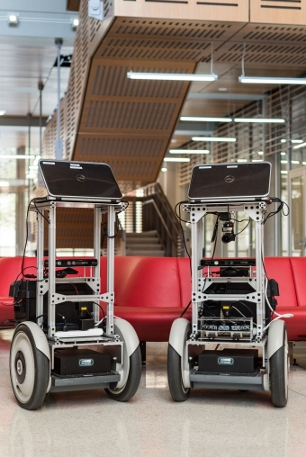
\includegraphics[width=\textwidth]{images/bwi3.png}
		\caption{Two SegBots from the Building-Wide Intelligence Project.}\label{fig:1a}		
	\end{subfigure}
    \begin{comment}
	\quad
	\begin{subfigure}[t]{2in}
		\centering
        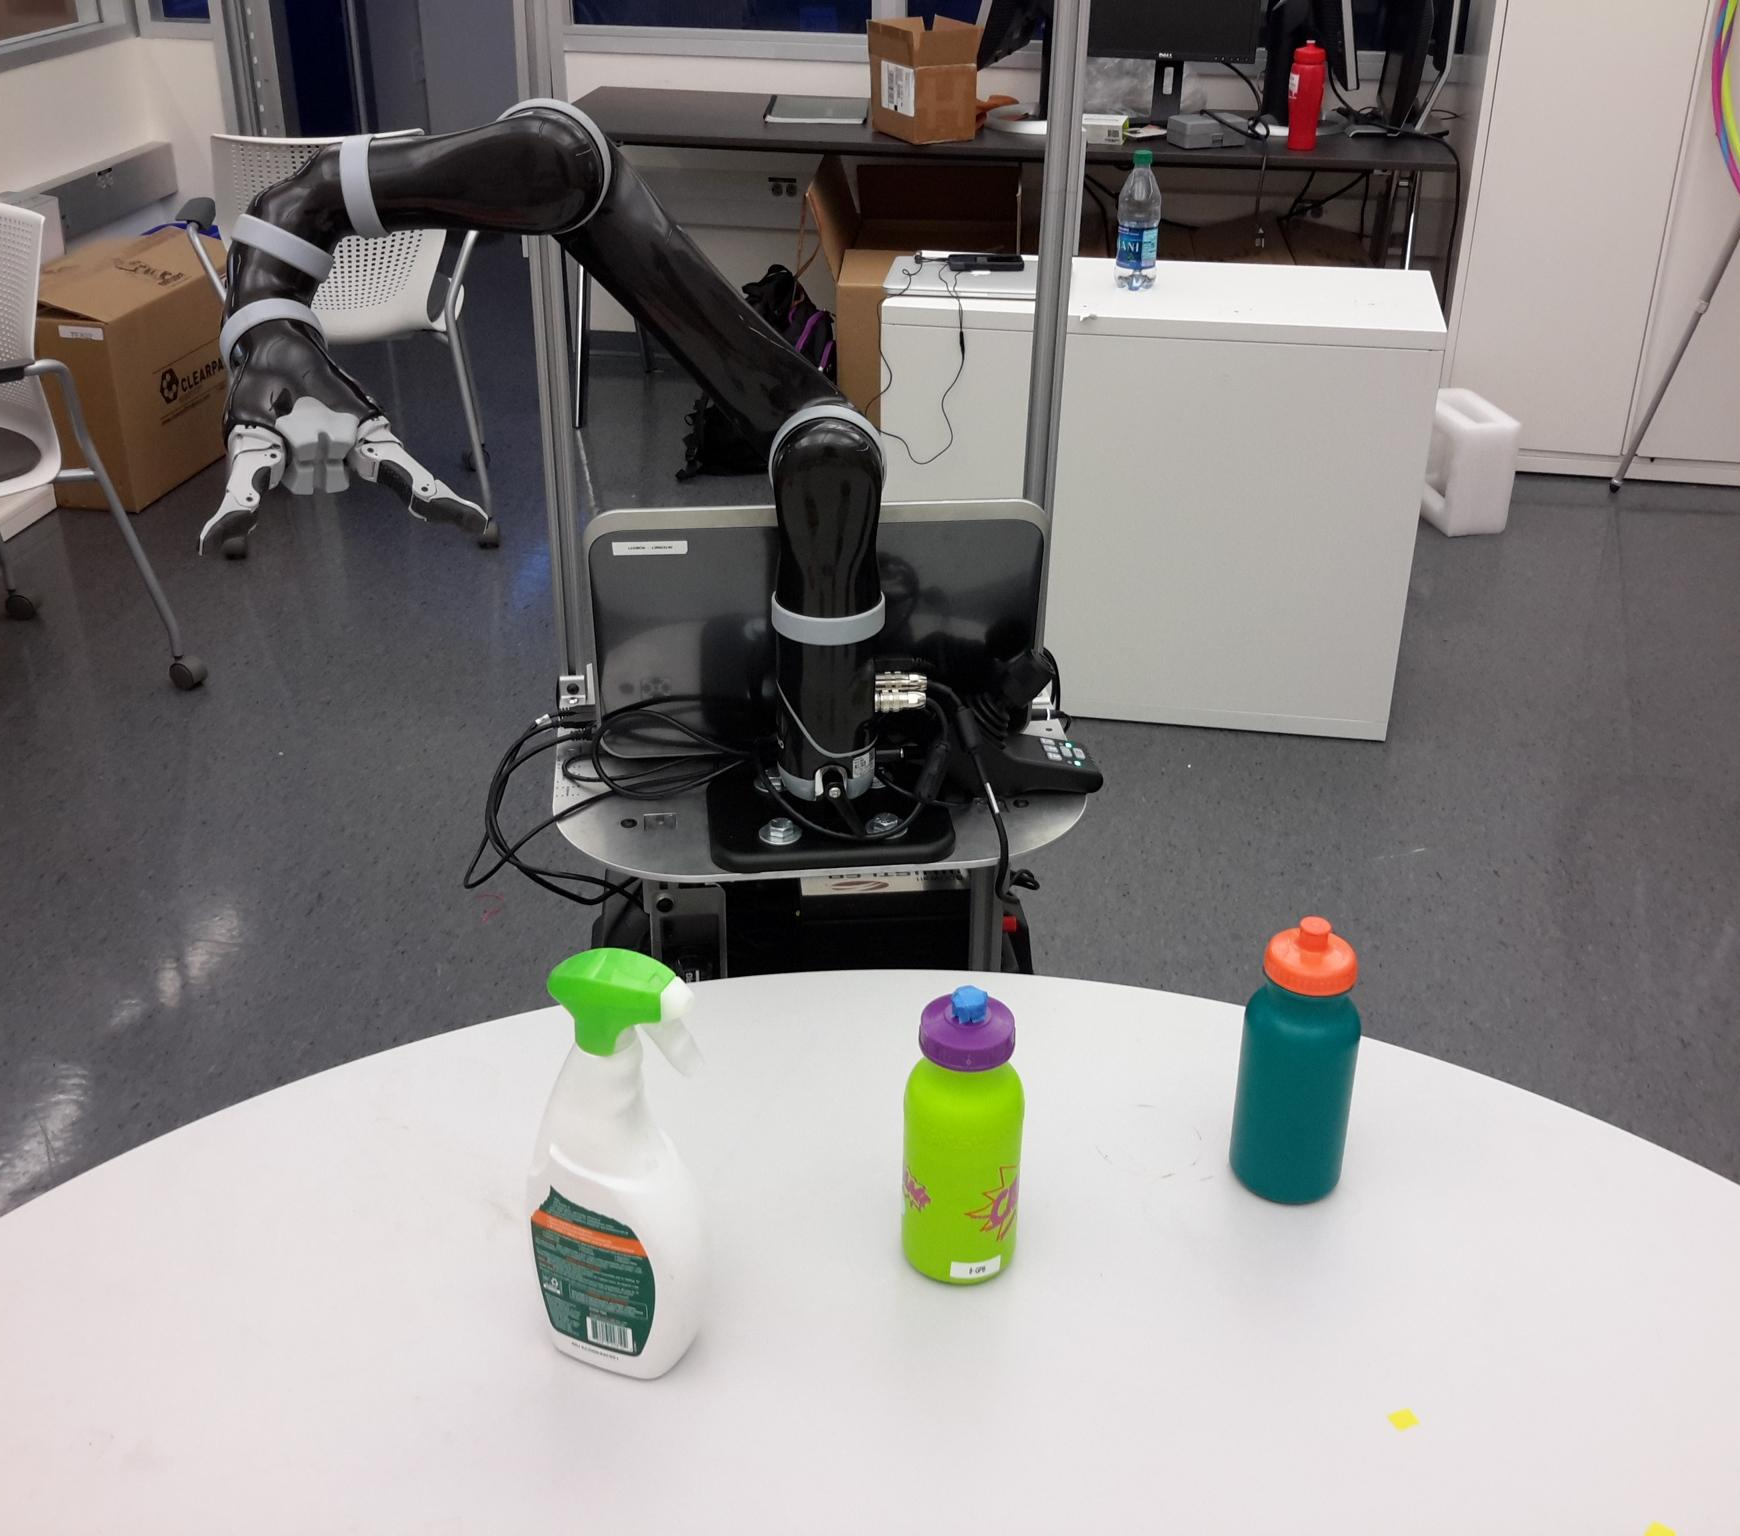
\includegraphics[width=\textwidth]{images/bwi_arm.png}
		\caption{SegBot with mounted Kinova Mico arm.}\label{fig:1b}
	\end{subfigure}
    \end{comment}
	\quad
	\begin{subfigure}[t]{1.4in}
		\centering
        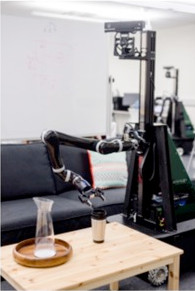
\includegraphics[width=\textwidth]{images/ut_poli.jpg}
		\caption{Custom robot used in Thomaz and Niekum's shared laboratory.}\label{fig:1c}
	\end{subfigure}
	\quad
	\begin{subfigure}[t]{1.4in}
		\centering
        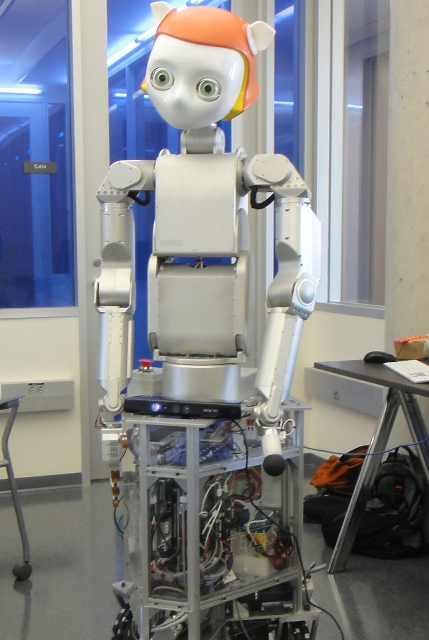
\includegraphics[width=\textwidth]{images/dreamer.png}
		\caption{Dreamer is a compliant humanoid robot used in Sentis's laboratory.}\label{fig:1d}
	\end{subfigure}
	\caption{Platforms in use by the UT Austin Villa RoboCup@Home Team.}\label{fig:1}
\end{figure*}


%The basic approach that our team is taking in the RoboCup@Home competition is to use development on the shared common platform of the Toyota HSR towards the RoboCup@Home competition as a means of integrating research across our laboratories.


Among the central goals of our research is the development of robotic systems capable of long-term autonomous human-robot interaction, automated planning, reasoning, and learning in complex real-world environments. By defining a novel competition framework situated within a domestic environment that uniquely exposes the challenges of this proposition, RoboCup@Home is an ideal setting for advancing the state of the art in long-term autonomy for human-interactive robots, and presents a both a task framework that is harmonized with our goals and a standard set of tasks against which we can compare our platform to other systems. With this motivation in mind, it is our goal to combine the competencies of our respective laboratories towards a full solution to the RoboCup@Home challenge, as well as to develop a common codebase which will allow our respective groups to interact more closely in our research activities. Our team brings together postdocs, graduate students, and undergraduate students from each of our groups to enable the robot to interact seamlessly with people in the environment, and to learn behaviors ranging from object manipulation to robust environmental perception to high-level task planning.

By leveraging our existing software and incorporating our HSR into our existing infrastructure, we hope to gain a jump start in developing our entry into the competition. We will also be able to make use of the infrastructure which we have in place for experiments on human-robot interaction in domestic and public spaces. Thomaz and Niekum's shared laboratory space is located in the same building as the BWI project, allowing us to test our system in both an open, interactive setting with many people to potentially interact with, and more controlled home-like settings. Prof. Sentis's laboratory is in a nearby building, and has a second HSR which will allow us to parallelize efforts more effectively, as we have a very large team. We expect that participation in the RoboCup@Home will boost our research efforts through collaboration between our groups, the sharing of ideas in an environment of friendly competition, and the advancements required to accomplish the tasks of the competition itself. We expect to make advancements on topics ranging from activity recognition, to robust perception, to learned planning and navigation, to general human-robot interaction.

%\section{Externally Available Components}

%Upon receiving the HSR robots, we will be able to ramp up quickly by building upon the extensive ROS ecosystem and other externally available software, as well as upon our existing BWI software infrastructure and our home-robotics research.

%Our own contributions to the growing ecosystem of externally available components, including a general architecture for service robots, robot reinforcement learning software, robot learning from demonstration software, and a package for tag-based perception are listed in Section~\ref{sec:reuse} below, with links on the application webpage.
